% Evidence-aware empirical results. Researcher-supplied exports: source origin and consent unverified.
\section{Experimental Evidence and Data Boundaries}

The research questions are evaluated separately before their proposed integration is considered. The supplied exports contain 32 businesses all classified as grocery/FMCG retail; 480 products in 16 categories; 365,447 order records; 561,152 shop--category--day observations; 72,146 historical customer snapshots; 2,500 offline policy scenarios; and 1,800 structured explanation cases. These are \emph{not} a validated cross-sector sample. Merchant source provenance, permission, and original collection process are not independently established. Later copies contain inconsistent synthetic metadata. Internal arithmetic consistency alone cannot authenticate the source. Raw customer records and row-level predictions must remain outside this public repository.

\subsection{Internal Source-Reconstruction Results}
A previously executed restricted audit matched the researcher-provided sales orders and line items to the 561,152-row daily panel, reporting zero value mismatches. It also reconstructed the provided 72,146 customer snapshots and found no discrepancy in the 90-day inactivity labels or selected temporal features. These checks are valuable internal arithmetic/temporal consistency evidence, but do not independently verify primary merchant origin or legal permission.

\section{RQ1: Demand Forecasting}

\subsection{Chronological Development and Refit}
RQ1 forecasts observed next-day shop--category sales, using only lagged demand and calendar predictors. The training period precedes 1 August 2025, validation covers August--September, and the reused test is October--December 2025 (47,104 rows). The historical test has already been inspected: results from newly tried models are exploratory, not estimates from a pristine, newly reserved model-selection holdout.

\begin{table}[htbp]\centering\small
\caption{RQ1 model comparison on the same 47,104 reused shop--category--day observations. Lower WAPE is better.}
\begin{tabular}{lrr}\toprule
Candidate & WAPE (\%) & MAE (units)\\\midrule
Seven-day seasonal naive & 110.45 & 2.841\\
Seven-day trailing mean & 89.70 & 2.307\\
Refit LightGBM & \textbf{83.98} & \textbf{2.160}\\
Two-stage hurdle: sale probability $\times$ positive quantity & 84.04 & 2.162\\
XGBoost fixed-parameter regressor & 84.56 & 2.175\\\bottomrule
\end{tabular}
\end{table}

Thus neither new candidate beats the original LightGBM on the same unit and period. There is no evidence here that adding a more complex model alone solves sparse-demand error. The original LightGBM fit and its re-execution agree to the displayed precision.

\subsection{Four-Level Forecast Aggregation Audit}
The identical LightGBM predictions were summed first, and the absolute differences were calculated \emph{after} aggregation at each level. Consequently these are \emph{four evaluations of the same forecasts}, not four separately trained models.

\begin{table}[htbp]\centering\small
\caption{Forecast accuracy evaluated at four levels on the same October--December 2025 predictions.}
\begin{tabular}{lrr}\toprule
Evaluation unit & Observations & WAPE (\%)\\\midrule
Network total per day & 92 & \textbf{6.02}\\
Individual shop total per day & 2,944 & 31.43\\
Product category total per day & 1,472 & 16.55\\
Shop $\times$ category per day & 47,104 & 83.98\\\bottomrule
\end{tabular}
\end{table}

At the most granular level, the sum of absolute errors is 101,752.89 units. After summing signed errors over each date and then taking absolute values, the sum is only 7,292.43 units. Therefore 92.83\% of the granular absolute-error mass cancels at the network/day level. A network/day WAPE of 6.02\% is not a shop-category or SKU forecast-accuracy claim. A network total is less informative for selecting an order quantity for an individual shop and product.

\begin{figure}[htbp]\centering
\IfFileExists{Figures/rq1_hierarchy_wape.png}{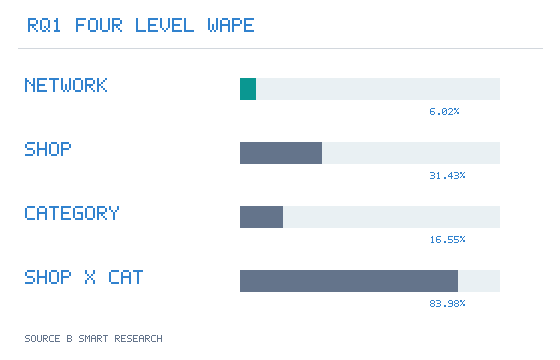
\includegraphics[width=0.88\textwidth]{Figures/rq1_hierarchy_wape.png}}{\fbox{\parbox{0.81\textwidth}{\centering Add the measured PNG to \texttt{Figures/rq1\_hierarchy\_wape.png}.}}}
\caption{RQ1 measured WAPE at four aggregation levels. The result uses the same LightGBM test predictions, not four distinct models.}
\end{figure}

\subsection{Zero Sales, Variability, and Shop/Category Heterogeneity}
There are 18,757 observed zero-sales rows (39.82\%) among 47,104 test rows. LightGBM predicts 1.708 units on average for those rows, although the observed volume is zero. WAPE is \emph{undefined} on a subset whose total observed demand is zero; MAE is 1.708 on that subset. The positive-observed-sales subset has WAPE 57.54\%. Neither observation distinguishes true zero demand from sales censored by stockouts. Reliable stock-level history is required.

Across the 512 shop--category series, larger zero-sales shares and higher coefficient-of-variation measures co-occur with higher WAPE. The descriptive Spearman associations were 0.984 and 0.972 respectively; their size may be mechanically amplified by small WAPE denominators and thus is \emph{not causal proof} that intermittency independently drives error. Per-shop and per-category diagnostics should be interpreted alongside absolute units, series volume, and product availability.

\subsection{Earlier Rolling-Origin Evaluation}
Three additional month-long test windows (all prior to the October--December period) were evaluated with earlier chronological training and validation segments.

\begin{table}[htbp]\centering\small
\caption{Earlier temporal folds: same shop--category target; WAPE percentages.}
\begin{tabular}{lrr}\toprule
Test month & LightGBM & Trailing seven-day mean\\\midrule
March 2025 & 72.89 & 78.30\\
May 2025 & 81.83 & 86.60\\
July 2025 & 85.84 & 88.75\\\bottomrule
\end{tabular}
\end{table}

The direction of the baseline improvement is stable in these folds, while the absolute error varies substantially. These folds do not replace external authentication or a future untouched validation period. No Croston/SBA/TSB result is claimed unless a correctly implemented and executed benchmark is supplied.

\section{RQ2: Ninety-Day Customer Inactivity Prediction}

The outcome is no qualifying purchase in the following 90 days, not marketing uplift. Training uses 40,499 eligible historical snapshots after exclusion of 10,483 overlapping-label training records; testing uses 21,164 later snapshots. Temporal embargo protects against overlap of label windows. Because the same customers can appear at multiple historical times, this tests later behaviour of represented customers, not an independent unseen-customer population.

\begin{table}[htbp]\centering\small
\caption{RQ2 previously executed inactivity risk-ranking comparison.}
\begin{tabular}{lr}\toprule
Model / score & PR-AUC\\\midrule
Recency rule & 0.6528\\
Logistic regression & 0.7346\\
LightGBM classifier & \textbf{0.7405}\\\bottomrule
\end{tabular}
\end{table}

The LightGBM--logistic difference is 0.0059, so its incremental superiority is modest. PR-AUC is not classification accuracy. A new aggregate TreeSHAP diagnostic was produced from 1,200 reproducibly sampled test snapshots, without publishing customer-level attribution: the largest mean absolute log-odds contributions were lifetime orders (1.088), orders in the preceding 180 days (0.447), tenure (0.357), and recency (0.277). These represent associations within the trained model, not causal effects or evidence of human understanding. Prospective contact consent and measured incremental retention impact remain necessary.

\begin{figure}[htbp]\centering
\IfFileExists{Figures/rq2_shap_global.png}{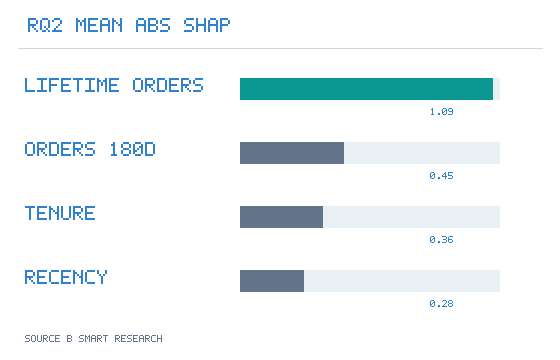
\includegraphics[width=0.88\textwidth]{Figures/rq2_shap_global.png}}{\fbox{\parbox{0.81\textwidth}{\centering Add \texttt{Figures/rq2\_shap\_global.png} from the offline experiment package.}}}
\caption{Aggregate LightGBM TreeSHAP attribution for RQ2; log-odds units, not causal importance.}
\end{figure}

\section{RQ3: Feasible Strategy and Cost--Service Analysis}

The provided policy-comparison export contains 2,500 synthetic-oracle scenarios; it is not connected by verified order records to RQ1 forecasts, actual lead-time demand, or observed stockout outcomes. Baseline simulated cost is BDT 2,227,690.07; trend simulated cost is BDT 2,208,289.47, a difference of BDT -19,400.60. Yet scenario lost units rise from 45 to 100. The trend policy is cheaper in 5.16\% of cases, equal in 94.80\%, and more expensive in 0.04\%.

For 97.68\% of scenarios, initial stock is already at least as high as the specified synthetic future 30-day demand (mean initial stock 156.54 units, mean future demand 3.33). This test is therefore dominated by low-action/high-stock cases, which limits its ability to discriminate policies. A credible next-stage RQ3 study requires a verified stock ledger, receipts, supplier lead time, cost definition, and comparable historical demand; evaluate holding/shortage/waste costs and service levels under a fixed matched replay. It must not infer realised savings from the synthetic oracle.

\section{RQ4: Recommendation Evidence and Explainability}

The provided 1,800 scenario-oriented explanation records contain 199 REORDER and 1,601 NO\_ACTION outcomes, with reasons: 1,600 sufficient-stock, 199 below-reorder-point with budget available, one budget-insufficient. All 1,800 records carry a supplied evidence-complete flag. This is a schema-completeness observation, not independent evidence verification. A model's SHAP feature contribution, a structured business constraint reason, and an SME owner's understanding are distinct validation targets. Human-participant response, decision correctness, completion time, and trust have \emph{not} been measured.

\section{Integrated Interpretation and Outstanding Validation}
\begin{enumerate}
\item \textbf{RQ1 + RQ3:} Forecast skill at the specific inventory decision unit and the full lead-time horizon must precede constrained policy optimisation. Network-level cancellation is not sufficient for product-level reorder decisions.
\item \textbf{RQ2 + RQ4:} Risk scores can prioritise review; explanation, consent, human comprehension, and later outcomes must be independently checked before intervention claims.
\item \textbf{Software boundary:} Offline trained models are not deployed as verified versioned production inference APIs.
\item \textbf{Generalisability:} The 32 provided stores are all grocery/FMCG; multi-sector usefulness is an intended design property, not empirically established.
\item \textbf{Integrity and ethics:} Raw-order reconciliation is a useful internal consistency check, but true merchant origin, lawful use, and participant permission require independent evidence.
\item \textbf{Publication validity:} Model additions and diagnostic choices made after inspecting the historical test are exploratory. Reserve a future period or external collection for final confirmation.
\end{enumerate}
